\begin{frame}{Water Restraints: Ion-Tethered vs. Excluded-from-Filter}
\begin{tikzpicture}
\pcuad{\textwidth}{\textheight}
%\showcuad
\path(nw) +(0,0) node(image)[anchor=north west]{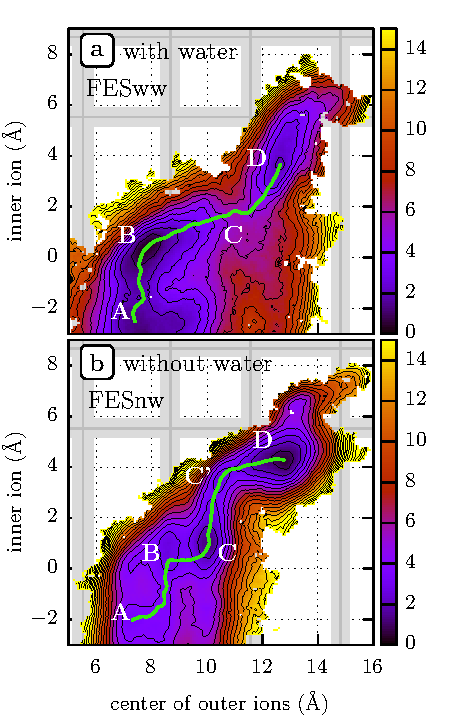
\includegraphics[width=0.5\textwidth]{wc_fes.pdf}};
\path(nw) +(5,-1.5) node(bullets)[anchor=north west,text width=0.5\textwidth]{\begin{itemize}
\item With one water tethered to each K$^+$, FES resembles unrestrained one
\item With water excluded from channel, ion motion is less concerted, more ``hard-knock'' like
\end{itemize}};
\end{tikzpicture}
\end{frame}

